\documentclass[tikz, usenames, dvipsnames]{standalone}
\usepackage{pgfplots}
\usepgfplotslibrary{groupplots}
\pgfplotsset{width=8.2cm, height=7cm, compat=1.18}
\usepackage{tikz}
\usepackage{gensymb}
\usepackage{amsmath}
\newcommand{\spminus}{^{\smash{-}}}
\usepackage[outline]{contour}
\contournumber{64}% default is 16, star form uses 32
\contourlength{.12em}% default is 0.03em
\usetikzlibrary {arrows.meta} 
\usetikzlibrary{decorations.pathreplacing, calligraphy}

\def\myline{very thick}
% psi = arctan (b sin phi / (a+b cos phi))
\def\psilow{0.89605}
\def\psihigh{1.190289}

\begin{document}
	
	
	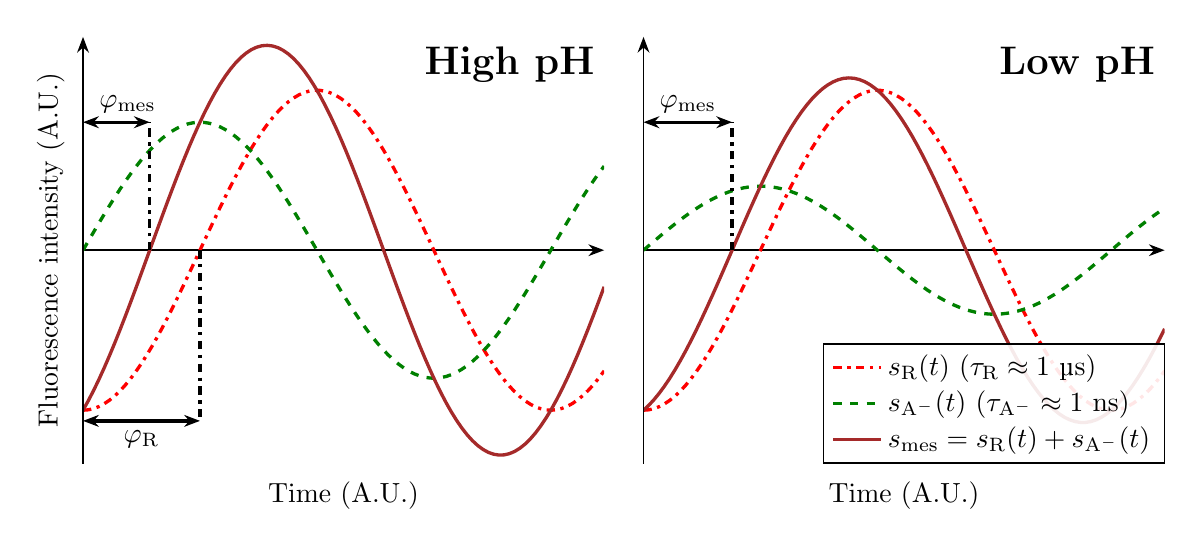
\begin{tikzpicture}
		%\draw[draw=black] (-1,-1) rectangle ++(14.5cm,7cm);
		\begin{groupplot}[group style={group size=2 by 1, horizontal sep=0.5cm}]
			%
			\nextgroupplot[
			legend cell align={left},
			tick align=outside,
			tick pos=left,
			xlabel={Time (A.U.)},
			xmin=0, xmax=7,
			xtick style={draw=none},
			xticklabels={},
			xlabel style={yshift=8pt},
			ylabel={Fluorescence intensity (A.U.)},
			ylabel style={yshift=-8pt},
			ymin=-1, ymax=1,
			ytick style={color=black},
			yticklabels={},
			ytick style={draw=none},
			axis line style={draw=none},
			clip mode=individual,
			domain=0:7,
			samples=100
			]
			\draw[-{Stealth[length=2mm]}, semithick] (0, 0) -- (7, 0); % xaxis
			
			\addplot[red, no marks, \myline, , dashdotted] {0.75*sin(180/pi*x - 90)};
			\addplot[Green, no marks, \myline, dashed] {0.6*sin(180/pi*x)};
			\addplot[Brown, no marks, \myline] {0.6*sin(180/pi*x) + 0.75*sin(180/pi*x - 90)};
			
			% phi mes stuff
			\draw[black, \myline, dashdotted] (\psilow, 0) -- (\psilow, 0.6);
			\draw[{Stealth[length=2mm]}-{Stealth[length=2mm]}, \myline] (0, 0.6) -- (\psilow, 0.6);
			\node[anchor=south] at (axis cs:\psilow/2+0.15, 0.6) {$\varphi_\text{mes}$};
			
			% phi R stuff
			\draw[black, \myline, dashdotted] (pi/2, 0) -- (pi/2, -0.8);
			\draw[{Stealth[length=2mm]}-{Stealth[length=2mm]}, \myline] (0, -0.8) -- (pi/2, -0.8);
			\node[anchor=north] at (axis cs:pi/4, -0.8) {$\varphi_\text{R}$};
			
			\draw[-{Stealth[length=2mm]}, semithick] (0,-1) -- (0,1); % yaxis
			
			\node[anchor=north east] at (axis cs:7, 1) {\Large{\textbf{High pH}}};
			
			\nextgroupplot[
			legend cell align={left},
			tick align=outside,
			tick pos=left,
			xlabel={Time (A.U.)},
			xmin=0, xmax=7,
			xtick style={draw=none},
			xticklabels={},
			xlabel style={yshift=8pt},
			ylabel style={draw=none},
			ymin=-1, ymax=1,
			ytick style={color=black},
			yticklabels={},
			ytick style={draw=none},
			axis line style={draw=none},
			clip mode=individual,
			domain=0:7,
			samples=100,
			legend style={
				fill opacity=.9,
				draw opacity=1,
				text opacity=1,
				at={(axis cs:7,-1.)},
				anchor=south east,
				draw=black
			},
			]
			\draw[-{Stealth[length=2mm]}, semithick] (0, 0) -- (7, 0); % xaxis
			
			\addplot[red, no marks, \myline, , dashdotted] {0.75*sin(180/pi*x - 90)};
			\addlegendentry{$s_\text{R}(t)$ ($\tau_\text{R} \approx 1$~\textmu{}s)}
			\addplot[Green, no marks, \myline, dashed] {0.3*sin(180/pi*x)};
			\addlegendentry{$s_\mathrm{A\spminus}(t)$ ($\tau_\mathrm{A\spminus}\approx 1$~ns)}
			\addplot[Brown, no marks, \myline] {0.3*sin(180/pi*x) + 0.75*sin(180/pi*x - 90)};
			\addlegendentry{$s_\text{mes} = s_\text{R}(t) + s_\mathrm{A\spminus}(t)$}
			
			% phi mes stuff
			\draw[black, \myline, dashdotted] (\psihigh, 0) -- (\psihigh, 0.6);
			\draw[{Stealth[length=2mm]}-{Stealth[length=2mm]}, \myline] (0, 0.6) -- (\psihigh, 0.6);
			\node[anchor=south] at (axis cs:\psihigh/2, 0.6) {$\varphi_\text{mes}$};
			
			\draw[-{Stealth[length=2mm]}, semithick] (0,-1) -- (0,1); % yaxis
			
			\node[anchor=north east] at (axis cs:7, 1) {\Large{\textbf{Low pH}}};
			
		\end{groupplot}
		
		
	\end{tikzpicture}
	
\end{document}